\documentclass[11pt,a4paper]{article}

\usepackage{titling}
\usepackage[hidelinks]{hyperref}
\usepackage{graphicx}
\usepackage{grffile}
\usepackage{float}
\usepackage{geometry}

\newcommand{\subtitle}[1]{
  \posttitle{
    \par\end{center}
    \begin{center}\large#1\end{center}
    \vskip0.5em}
}

\begin{document}


\title{Hyper Perform\\ Functional Requirements Specification}
\subtitle{ Repository: \url{https://github.com/claudioMDS/hyper-perform}}
\begin{figure}
			\centering
			
\includegraphics[height=200px]{../Images/CodusMaximus_logo.jpg}
\end{figure}

	
\author{
	\textbf{Developers:} \\
	Claudio Da Silva	\emph{14205892}	\\
	Rohan Chhipa		\emph{14188377}	\\
	Avinash Singh		\emph{14043778}	\\
	Jason Gordon		\emph{14405025}	\\\\
}

\date{\textbf{Updated \today}}

\maketitle
\thispagestyle{empty}
\pagebreak

\tableofcontents
\pagebreak

\section{Introduction}
Many different tools are available for measuring the quality of products made, but very few tools exist which assess the quality of the people making said products. People play a huge role in a project, and trying to monitor each and every one becomes a tedious task which diverts man power away from other more critical tasks. Whether it be for an end of year evaluation, or attempting to assess the current status of a project, generating a report on a staff member can help keep up productivity, as well as get them any help they need in order to resume quality performance. By ensuring that there is constant quality performance from each individual on a project, one can increase project quality as well as reduce project risks such as loss of an important team member during a critical stage of a project's life-cycle. 

\section{Vision and Objectives}
\subsection{Vision}
The vision of this project is to create an automated performance management system, which can assess the performance and status of staff members, based on information sourced through various software systems such as card readers, version control systems and such. The system would make use of these external integrations as well as direct contact with the staff members via either web dashboard or mobile phone, to generate reports on the various staff members as well as add elements such as gamification and monitor problems that may be occurring.

\subsection{Objectives}
The objectives for the Hyper Perform system are:
\begin{itemize}
	\item To source information from various forms of software systems and transform it into usable data to determine performance.
	\item To generate real-time reports on staff members in order to evaluate performance based on this data.
	\item To monitor staff members in order to determine possible causes of work detriment.
	\item To add a form of gamification to encourage productivity, and discourage slacking and other bad behaviours.

\end{itemize}



\section{User Management}
\subsection{Scope}
\begin{figure}[H]
	\begin{center}
		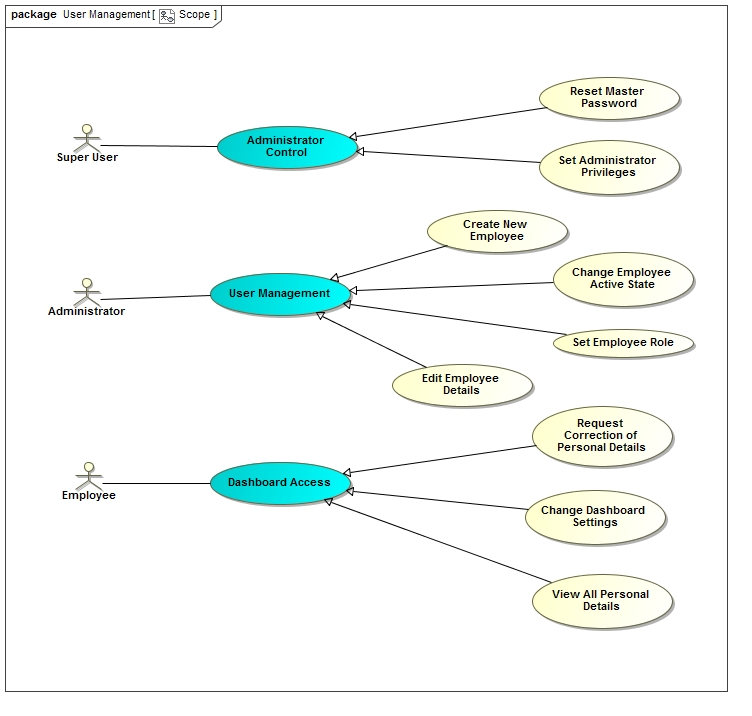
\includegraphics[scale=0.6]{../Images/User_Management_Scope.jpg}
		\caption{User Management Scope}
	\end{center}
\end{figure}

\pagebreak

The scope of the user management module includes:
\begin{itemize}
	\item Super user control over administrator rights given to individuals.
	\item Administrators may add employees and manage their details.
	\item Administrators may add employee roles to employees registered, which will define which algorithms and systems will influence their performance ratings.
	\item A user may change their dashboard to reflect what the wish to see.
	\item A user should be able to view all their personal details, and request change immediately if something is wrong. 
\end{itemize}
Note, it is assumed that a super user is not in anyway an employee within the system. It is also assumed that an Administrator is automatically an employee of the system. Administrators may not review themselves or change their own details, such action must be authorised by another administrator.

\subsection{Domain Model}
\begin{figure}[H]
	\begin{center}
		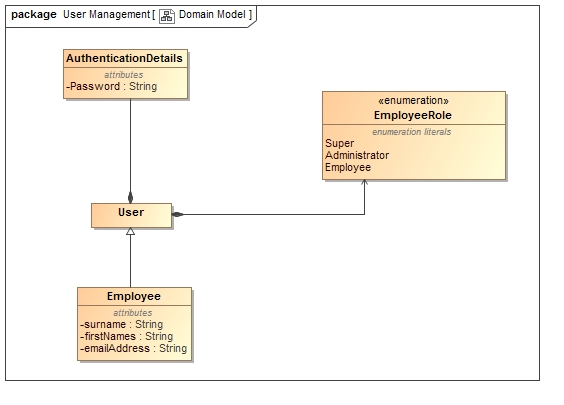
\includegraphics[scale=0.75]{../Images/User_Domain.jpg}
		\caption{User Management Domain Model}
	\end{center}
\end{figure}

\pagebreak

\section{Integration and Pre-processing}
\subsection{Scope}
\begin{figure}[H]
	\begin{center}
		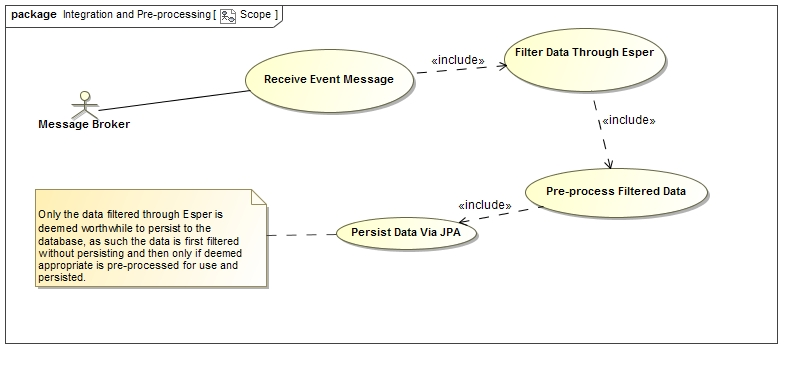
\includegraphics[scale=0.6]{../Images/Integration_Scope.jpg}
		\caption{Integration and Pre-processing Scope}
	\end{center}
\end{figure}
The scope of the integration module includes:
\begin{itemize}
	\item Events are received through a REST URL that is made available to the services. There is no need for polling these systems.
	\item Each event is converted to a Java object and is persisted. Along with being persisted each event object is also placed onto a message queue where Esper will act as the consumer on the other end.
	\item Algorithms are applied to the persisted data to generate reports.
\end{itemize}

\subsection{Domain Model}
\begin{figure}[H]
	\begin{center}
		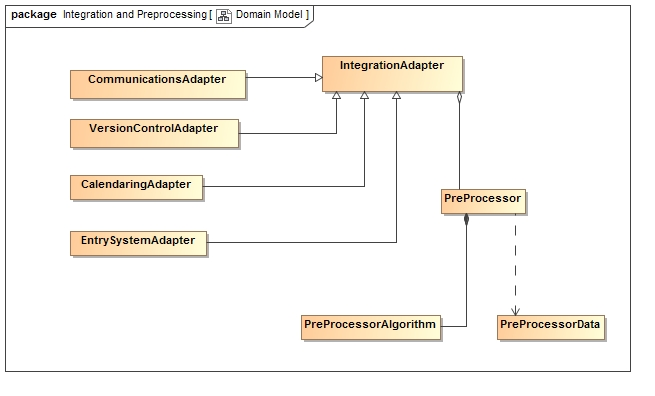
\includegraphics[scale=0.75]{../Images/Integration_Domain.jpg}
		\caption{Integration and Pre-processing Domain Model}
	\end{center}
\end{figure}

\pagebreak

\section{Algorithms}
\subsection{Scope}
\begin{figure}[H]
	\begin{center}
		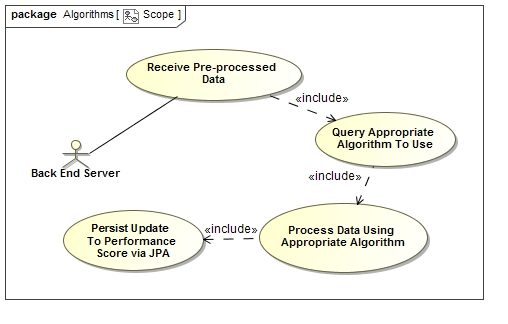
\includegraphics[scale=0.75]{../Images/Algorithms_Scope.jpg}
		\caption{Algorithms Scope}
	\end{center}
\end{figure}
The scope of the algorithms module includes:
\begin{itemize}
	\item Determining which algorithm "recipe" will be appropriate in the current circumstance.
	\item Applying said "recipe" to the data provided, and then updating the employee in question's performance score accordingly.
\end{itemize}

\subsection{Domain Model}
\begin{figure}[H]
	\begin{center}
		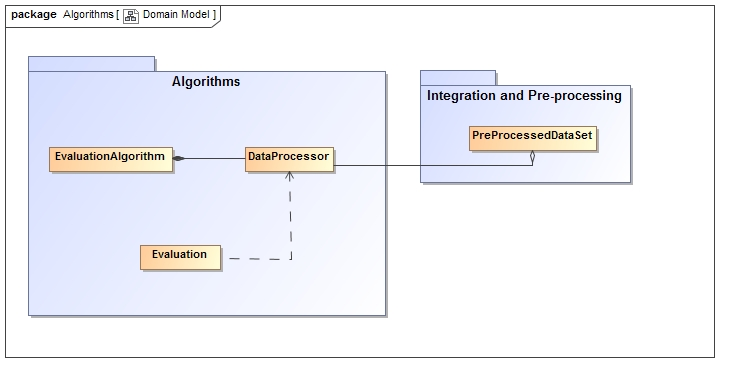
\includegraphics[scale=0.6]{../Images/Algorithm_Domain.jpg}
		\caption{Algorithms Domain Model}
	\end{center}
\end{figure}

\pagebreak

\section{Reporting}
\subsection{Scope}
\begin{figure}[H]
	\begin{center}
		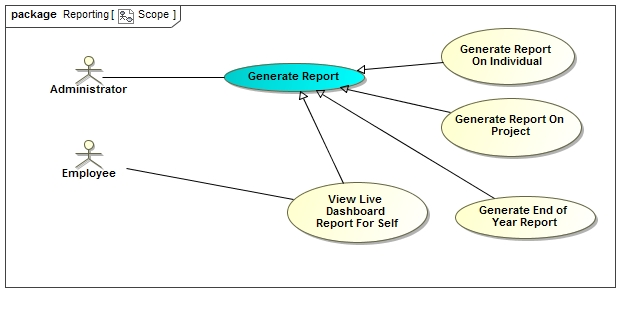
\includegraphics[scale=0.75]{../Images/Reporting_Scope.jpg}
		\caption{Reporting Scope}
	\end{center}
\end{figure}
The scope of the reporting module includes:
\begin{itemize}
	\item Administrators such as HR may request reports on individual employee's performance.
	\item Administrators may also request reports on the current project performance, as well as an end of year final report.
	\item All users, including administrators whom are users, may view their own dashboard which contains information regarding their current performance and personal details.
\end{itemize}

\subsection{Domain Model}
\begin{figure}[H]
	\begin{center}
		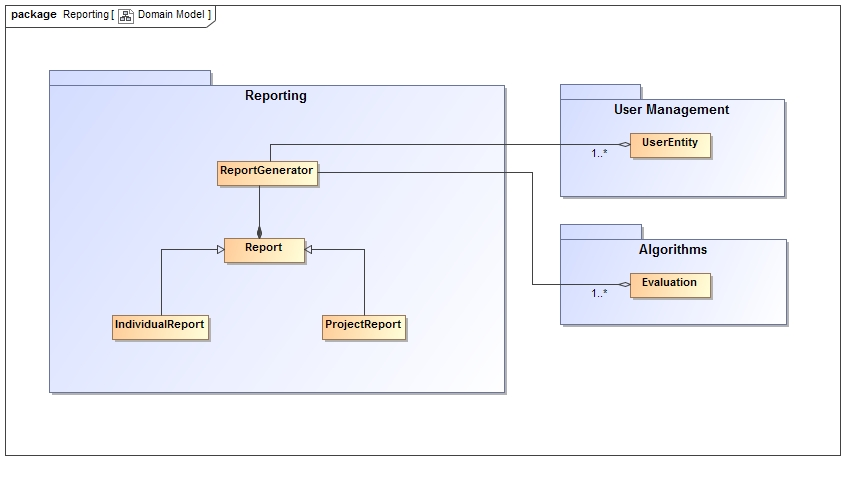
\includegraphics[scale=0.55]{../Images/Report_Domain.jpg}
		\caption{Reporting Domain Model}
	\end{center}
\end{figure}

\pagebreak

\section{Notifications}
\subsection{Scope}
\begin{figure}[H]
	\begin{center}
		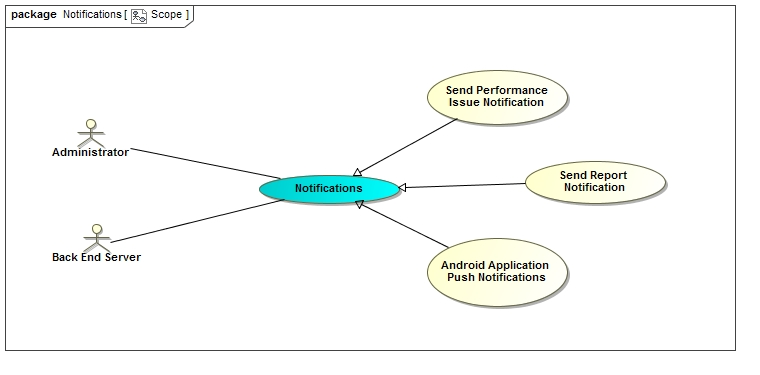
\includegraphics[scale=0.6]{../Images/Notifications_Scope.jpg}
		\caption{Notifications Scope}
	\end{center}
\end{figure}
The scope of the notifications module includes:
\begin{itemize}
	\item Sending a notification about a rapid decline in performance.
	\item Send a notification about a report that an employee requests.
	\item Push notifications are sent to the Android device to notify of important events or required surveys.
\end{itemize}

\subsection{Domain Model}
\begin{figure}[H]
	\begin{center}
		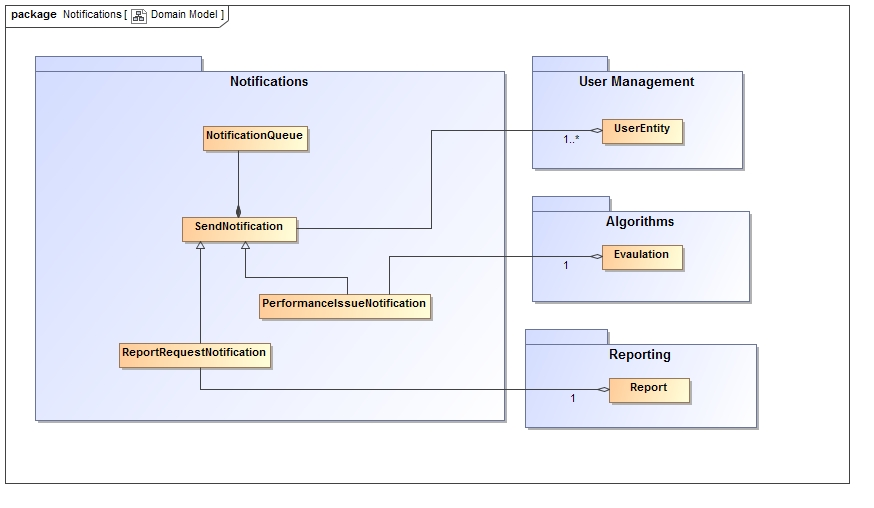
\includegraphics[scale=0.55]{../Images/Notifications_Domain.jpg}
		\caption{Notifications Domain Model}
	\end{center}
\end{figure}



\end{document}